%\documentclass[a4paper,pdf]{article} % gebruik acm style voor je scriptie: [format=acmsmall, screen=true, review=false]{acmart} 
%### ACM template on overleaf

%* You can find the ACM template also on overleaf. You can then use the points below for the content.
%* <https://www.overleaf.com/latex/templates/acm-conference-proceedings-master-template/pnrfvrrdbfw>


%\documentclass[sigconf]{acmart} 
\documentclass[sigconf,format=acmsmall, screen=true, review=false]{acmart} 
\usepackage{amsmath}
\usepackage{amsfonts}
\usepackage{amssymb}
\usepackage{hyperref}
\usepackage{pdfpages} % http://mirror.unl.edu/ctan/macros/latex/contrib/pdfpages/pdfpages.pdf
\usepackage{booktabs} 


\usepackage[utf8]{inputenc}
\usepackage{graphicx}
\usepackage[colorinlistoftodos]{todonotes} % handig voor commentaar: gebruik \todo{}, zie ftp://ftp.fu-berlin.de/tex/CTAN/macros/latex/contrib/todonotes/todonotes.pdf
\usepackage{listings}
 
\usepackage{tcolorbox}
\usepackage{float}
\usepackage{caption}
\usepackage{subcaption}


% when writing in Dutch
%\usepackage[dutch]{babel}
%\selectlanguage{dutch}


% linenumbering  See https://texblog.org/2012/02/08/adding-line-numbers-to-documents/
\usepackage{lineno}
\linenumbers

\newcommand{\shorttitle}{} % Put your short title here
\begin{document}




%%%% DIT IS DE TITLE PAGE VOOR INFORMATIEKUNDE NIET VOOR AI OF INFORMATICA! 
%% GEBRUIK VOOR AI OF INFORMATICA JE EIGEN TITLEPAGE TEMPLATES\


\begin{center}

\vspace{2.5cm}

% [CHANGE] The title of your thesis. If your thesis has a subtitle, then this
% should appear right below the main title, in a smaller font.
\begin{Huge}
Title of the thesis
\end{Huge}

\vspace{1.5cm}

% [CHANGE] Your full name. In case of multiple names, you can include their
% initials as well, e.g. "Jan G.J. van der Wegge".
Jan van der Wegge\\
% [CHANGE] Your student ID, as this has been assigned to you by the UvA
% administration.
9123456

\vspace{1.5cm}

% [DO NOT CHANGE]
Bachelor thesis\\
% [CHANGE] Whether your Bachelor thesis is 6 ECTS (regular) or 9 ECTS (Honours
% programme).
Credits: 12 EC

\vspace{0.5cm}

% [DO NOT CHANGE] The name of the educational programme.
Bachelor Opleiding Informatiekunde

\vspace{0.25cm}

% [DO NOT CHANGE] The addess of the educational programme.
University of Amsterdam\\
Faculty of Science\\
Science Park 904\\
1098 XH Amsterdam

\vspace{4cm}

\emph{Supervisor}\\
% [CHANGE] The name of your supervisor. Include the titles of your supervisor,
% as well as the initials for *all* of his/her first names.
Dr. M. J. Marx

\vspace{0.25cm}

% [CHANGE] The address of the institute at which your supervisor is working.
% Be sure to include (1) institute (is appropriate), (2) faculty (if
% appropriate), (3) organisation name, (4) organisation address (2 lines).
ILPS, IvI\\
Faculty of Science\\
University of Amsterdam\\
Science Park 904\\
1098 XH  Amsterdam

\vspace{1.5cm}

% [CHANGE] The date at which you will finalize and submit your thesis.
2016-06-26

\end{center}

%\documentclass[]{article}
%\usepackage{lmodern}
%%\usepackage{fontspec}
%\usepackage{amssymb,amsmath}
%\usepackage{ifxetex,ifluatex}
%\usepackage{fixltx2e} % provides \textsubscript
%\ifnum 0\ifxetex 1\fi\ifluatex 1\fi=0 % if pdftex
%  \usepackage[T1]{fontenc}
%  \usepackage[utf8]{inputenc}
%\else % if luatex or xelatex
%  \ifxetex
%    \usepackage{mathspec}
%    \usepackage{xltxtra,xunicode}
%  \else
%    \usepackage{fontspec}
%  \fi
%  \defaultfontfeatures{Mapping=tex-text,Scale=MatchLowercase}
%  \newcommand{\euro}{€}
%\fi
%% use upquote if available, for straight quotes in verbatim environments
%\IfFileExists{upquote.sty}{\usepackage{upquote}}{}
%% use microtype if available
%\IfFileExists{microtype.sty}{%
%\usepackage{microtype}
%\UseMicrotypeSet[protrusion]{basicmath} % disable protrusion for tt fonts
%}{}
%\usepackage{graphicx}
%\makeatletter
%\def\maxwidth{\ifdim\Gin@nat@width>\linewidth\linewidth\else\Gin@nat@width\fi}
%\def\maxheight{\ifdim\Gin@nat@height>\textheight\textheight\else\Gin@nat@height\fi}
%\makeatother
%% Scale images if necessary, so that they will not overflow the page
%% margins by default, and it is still possible to overwrite the defaults
%% using explicit options in \includegraphics[width, height, ...]{}
%\setkeys{Gin}{width=\maxwidth,height=\maxheight,keepaspectratio}
%\ifxetex
%  \usepackage[setpagesize=false, % page size defined by xetex
%              unicode=false, % unicode breaks when used with xetex
%              xetex]{hyperref}
%\else
%  \usepackage[unicode=true]{hyperref}
%\fi
%\hypersetup{breaklinks=true,
%            bookmarks=true,
%            pdfauthor={},
%            pdftitle={},
%            colorlinks=true,
%            citecolor=blue,
%            urlcolor=blue,
%            linkcolor=magenta,
%            pdfborder={0 0 0}}
%\urlstyle{same}  % don't use monospace font for urls
%\setlength{\parindent}{0pt}
%\setlength{\parskip}{6pt plus 2pt minus 1pt}
%\setlength{\emergencystretch}{3em}  % prevent overfull lines
%\setcounter{secnumdepth}{0}
%
%\date{}
%
%\begin{document}


\begin{titlepage}


\begin{center}
 
\textsc{\Large   Your Title }

\bigskip

\textsc{\large
submitted in partial fulfillment for the degree of master of science\\
%
\bigskip
Your Student Name\\
%
Your Student ID\\
%
\bigskip
master information studies\\
%
data science \\
%
faculty of science\\
%
university of amsterdam\\
%
\bigskip
Your Date of defence in the format YYYY-MM-DD
}

\end{center}
 
\vfill

\begin{center}
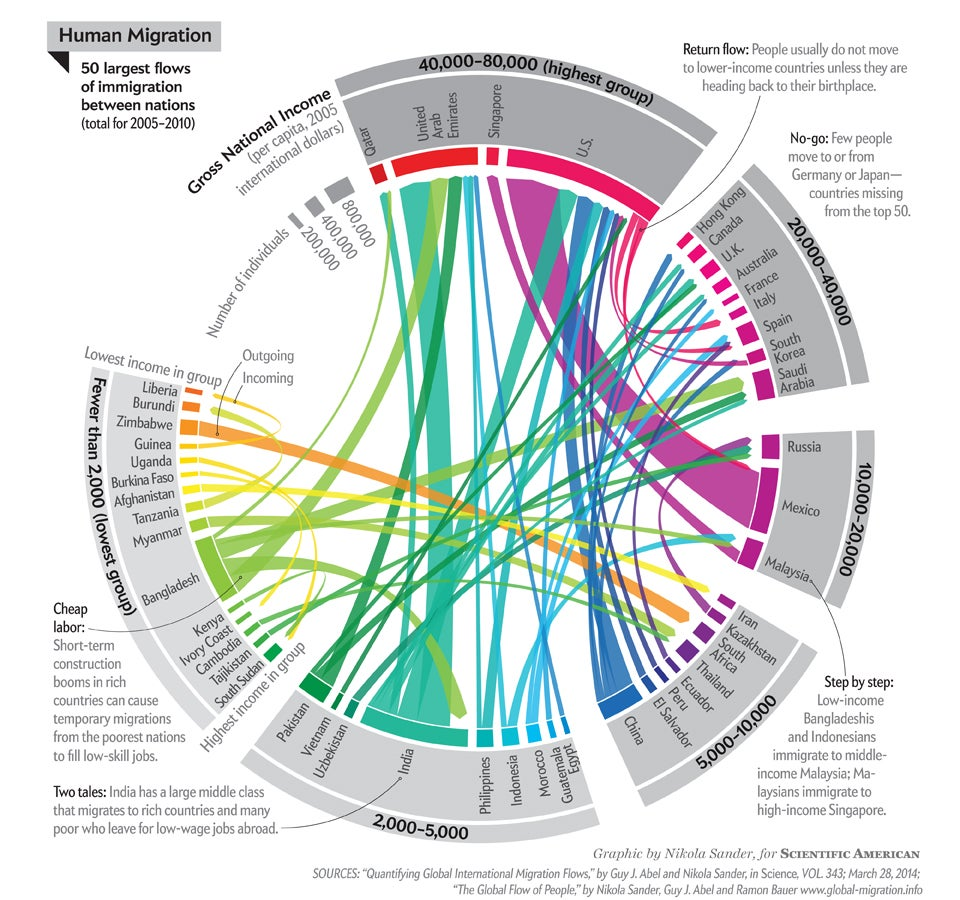
\includegraphics[height=.4\textheight]{TitlePages/logos/cover.jpeg} %width=\linewidth
\end{center}

\vfill

% In case of an internal project, remove External Supervisor or if you had two internal supervisors, change the header into 
%  & First Supervisor & Second Supervisor  \\
\begin{center}
\begin{tabular}{|l||ll|}
\hline
 & \textbf{Internal  Supervisor} & \textbf{External   Supervisor}  \\   
 \hline
\textbf{Title, Name} & Dr Maarten Marx&  \\
\textbf{Affiliation} &UvA, FNWI, IvI & \\ 
\textbf{Email} & maartenmarx@uva.nl& . \\
\hline
\end{tabular}
\end{center}



%% If you have a third supervisor use this table instead
%\begin{center}
%\begin{tabular}{|l||lll|}
%\hline
% & \textbf{External   Supervisor} & \textbf{External   Supervisor} & \textbf{3$^{\mathrm{rd}}$ supervisor} \\
% \hline
%\textbf{Title, Name} & Dr Maarten Marx& & \\
%\textbf{Affiliation} &UvA, FNWI, IvI & & \\ 
%\textbf{Email} & maartenmarx@uva.nl& &  .\\
%\hline
%\end{tabular}
%\end{center}

\bigskip

% logos
\begin{center}
\mbox{
\includegraphics[width=.2\paperwidth]{TitlePages/logos/logo-uva.png} 

\includegraphics[width=.2\paperwidth]{TitlePages/logos/ads.png}

\includegraphics[width=.2\paperwidth]{TitlePages/logos/ads.png} % replace by the logo of your internship company or remove
}
\end{center}
\end{titlepage}

%
%\newpage
%
%\end{document}
  % or use another template

\pagebreak

%\todototoc
%\listoftodos
%\tableofcontents

\pagebreak

\begin{abstract}
% [CHANGE] 
\end{abstract}


\section*{Thesis requirements}
\begin{itemize}
\item Your thesis is written in ACM style with two columns  (\texttt{documentclass[sigconf]{acmart}}).
\item   The	size	 of	a	18	EC master	thesis	is	set	at	10	pages	according	to	the	standards	used	for	ACM	and	IEEE	 conferences	 including	 the	 bibliography and	 acknowledgements,	 but excluding	 the	 cover	 page and	appendices.
\item Use one of the conference proceedings available from \url{https://www.acm.org/publications/proceedings-template}
\item Most proceedings authors (including ICPS authors) will use the "sigconf" proceedings template.
\item Use the template at \url{https://github.com/maartenmarx/ThesisTemplate/blob/master/ThesisTemplate/TitlePages/Thesis-Title-Page-DS.tex} for your titlepage.
\end{itemize}


\pagebreak


% Here you input all your sections in seperate files

\section{Introduction}
\label{sec:intro}
\begin{itemize}
\item Bevat je onderzoeksvraag (of vragen)
\item Plaatst je vraag in de bestaande literatuur.
\end{itemize}

Je onderzoeksvraag is leidend voor je hele scriptie. Alles wat je doet moet uiteindelijk terug te voeren zijn op 1 doel: het beantwoorden van die vraag. 

Typisch zal je het dan ook zo doen:

Mijn onderzoeksvraag is onderverdeeld in de volgende deelvragen:

\begin{description}
\item[RQ1] \ldots We   beantwoorden deze vraag  door het volgende te doen/ antwoord op de volgende vragen te vinden/ \ldots
\begin{enumerate}
\item Vragen op dit niveau kan je echt beantwoorden, en dat doe je in je Evaluatie sectie~\ref{sec:eva}.
\end{enumerate}
\item[RQ2] \ldots
\item[RQ3] \ldots
\end{description}
%
Je Evaluatie sectie~\ref{sec:eva} bevat evenveel subsecties als je deelvragen hebt. En in elke sectie beantwoord je dan die deelvraag met behulp van de vragen op het onderste niveau.

In je conclusies kan je dan je hoofdvraag gaan beantwoorden op basis van al het eerder vergaarde bewijs.


\paragraph{Overview of thesis}
Hier geef je even kort weer wat in elke sectie staat.
\section{Related Work}
\label{sec:rel}

Deze sectie bestaat uit een aantal "blokken", waarin je per blok de relevante literatuur beschrijft. 

Neem alleen literatuur op die van belang is voor jouw onderzoeksvraag en deelvragen.

Typisch heb je 1 blok voor je hoofdvraag en per deelvraag \textbf{RQi} een blok. 


\subsection{RQ1}

\subsection{RQ2}
\section{Methodology}
\label{sec:meth}


\subsection{Description of the data}
Data verzameling en beschrijving van de data

Hoe is de data verzameld, en hoe heb jij die data verkregen?


Wat staat er in de data? Niet alleen maar een technisch verhaal, maar ook inhoudelijk. DE lezer moet een goed idee krijgen over de technische inhoud en wat het betekent.

\pagebreak
\subsection{Wat plotjes en tabelletjes}

Zie het IPython Notebook \url{PandasAndLatex.ipynb} voor de code om vanuit pandas een poltje op te slaan en een dataframe als tabel op te slaan. Het werkt ideaal! 

De interrupties van Wilders staan beschreven in Figure~\ref{fig:wilders} en Tabel~~\ref{tab:Wilders}.


\begin{figure}
\begin{center}
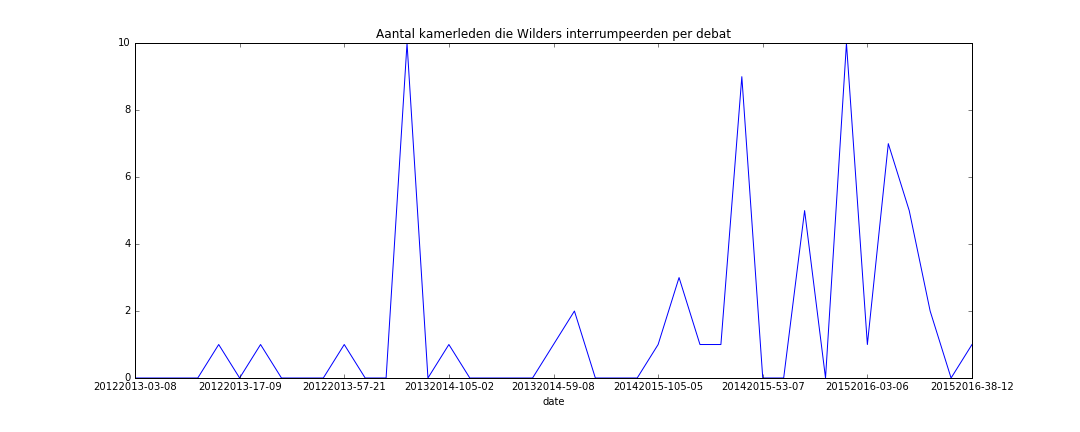
\includegraphics[width=\linewidth]{WildersPlot.png}
\caption{\label{fig:wilders} Aantal interrupties van Wilders in de Tweede Kamer door de tijd (periode 2012-2016).}
\end{center}
\end{figure}


\pagebreak

\begin{table}[h]
\begin{footnotesize}
\begin{tabular}{lrl}
\toprule
{} &  indegree &                               interruptie\_volgorde \\
date            &           &                                                    \\
\midrule
20122013-03-08  &       0.0 &                                                    \\
20122013-07-16  &       0.0 &                                                    \\
20122013-100-03 &       0.0 &                                                    \\
20122013-100-06 &       0.0 &                                                    \\
20122013-17-06  &       1.0 &                                         Pechtold-3 \\
20122013-17-09  &       0.0 &                                                    \\
20122013-21-04  &       1.0 &                                         Pechtold-3 \\
20122013-22-08  &       0.0 &                                                    \\
20122013-32-06  &       0.0 &                                                    \\
20122013-48-23  &       0.0 &                                                    \\
20122013-57-21  &       1.0 &                                         Pechtold-6 \\
20122013-76-03  &       0.0 &                                                    \\
20122013-76-06  &       0.0 &                                                    \\
20132014-05-02  &      10.0 &  Roemer-4 Van Haersma Buma-4 Pechtold-4 Slob-5 ... \\
20132014-06-04  &       0.0 &                                                    \\
20132014-105-02 &       1.0 &                                        Pechtold-10 \\
20132014-105-06 &       0.0 &                                                    \\
20132014-14-03  &       0.0 &                                                    \\
20132014-14-06  &       0.0 &                                                    \\
20132014-52-18  &       0.0 &                                                    \\
20132014-59-08  &       1.0 &                                           Klaver-3 \\
20142015-02-08  &       2.0 &                                  Pechtold-6 Slob-4 \\
20142015-03-06  &       0.0 &                                                    \\
20142015-09-09  &       0.0 &                                                    \\
20142015-100-05 &       0.0 &                                                    \\
20142015-105-05 &       1.0 &                                         Pechtold-2 \\
20142015-111-04 &       3.0 &                         Pechtold-6 Kuzu-8 Klaver-3 \\
20142015-111-07 &       1.0 &                                         Pechtold-2 \\
20142015-39-71  &       1.0 &                                         Pechtold-2 \\
20142015-41-07  &       9.0 &  Samsom-2 Pechtold-3 Kuzu-6 Zijlstra-5 Van Ojik... \\
20142015-53-07  &       0.0 &                                                    \\
20142015-61-23  &       0.0 &                                                    \\
20142015-79-07  &       5.0 &  Klaver-10 Gesthuizen-3 Voordewind-2 Pechtold-6... \\
20142015-95-06  &       0.0 &                                                    \\
20152016-02-07  &      10.0 &  Pechtold-5 Slob-7 Klaver-11 Kuzu-24 Öztürk-1 S... \\
20152016-03-06  &       1.0 &                                         Pechtold-5 \\
20152016-14-02  &       7.0 &  Klaver-9 Roemer-4 Samsom-2 Van Haersma Buma-5 ... \\
20152016-14-05  &       5.0 &  Van Haersma Buma-13 Pechtold-4 Zijlstra-1 Klav... \\
20152016-27-03  &       2.0 &                                   Segers-4 Kuzu-10 \\
20152016-38-10  &       0.0 &                                                    \\
20152016-38-12  &       1.0 &                                            Klein-2 \\
\bottomrule
\end{tabular}

\end{footnotesize}
\caption{\label{tab:Wilders} Door wie werd Wilders onderbroken en hoe vaak per debat.}
\end{table}


\pagebreak
\subsection{Methods}
Hoe je je vraag gaat beantwoorden.


Dit is de langste sectie van je scriptie. 

Als iets erg technisch wordt kan je een deel naar de Appendix verplaatsen. 

Probeer er een lopend verhaal van te maken.

Het is heel handig dit ook weer op te delen nav je deelvragen:

\subsubsection{RQ1}

\subsubsection{RQ2}
\section{Evaluation}
\label{sec:eva}

Met een subsectie voor elke deelvraag.

In hoeverre is je vraag beantwoord?

Een mooie graphic/visualisatie is hier heel gewenst.

Hou het kort maar krachtig.
\section{Conclusions}
\label{sec:conc}

Hierin beantwoord je jouw hoofdvraag op basis van het eerder vergaarde bewijs.



\subsection{Acknowledgements}
Hier kan je bedanken wie je maar wilt.

% your refs

\bibliographystyle{plain}
\bibliography{MyThesis}

\appendix

%\input{appendix}


\section{Slides}

% Example

\includepdf[nup=2x3 , pages=-]{sargent-lecture_slides.pdf}
 
\end{document}
